\documentclass[a4paper, 10pt, conference]{article}

\usepackage{graphics} % for pdf, bitmapped graphics files
\graphicspath{ {./plots/} }
\usepackage{epsfig} % for postscript graphics files
\usepackage{mathptmx} % assumes new font selection scheme installed
\usepackage{times} % assumes new font selection scheme installed
\usepackage{amsmath} % assumes amsmath package installed
\usepackage{amssymb}  % assumes amsmath package installed
\usepackage{color}
\usepackage{float}
\usepackage{hyperref}
\usepackage{booktabs}

\usepackage[margin=1in]{geometry}


\newcommand{\ttt}{\texttt}
\newcommand{\TODO}{{\color{red}\textbf{TODO}}}
\newcommand{\TODOx}[1]{{\color{red}\textbf{TODO: #1}}}


\newcommand{\LSTMenc}{\text{LSTMenc}}
\newcommand{\LSTMdec}{\text{LSTMdec}}
\newcommand{\BiLSTM}{\text{BiLSTM}} 
\newcommand{\HMN}{\text{HMN}}
\newcommand{\HMNstart}{\text{HMNstart}} % Please make this prettier -K
\newcommand{\HMNend}{\text{HMNend}}
\newcommand{\softmax}{\text{softmax}}

\setlength{\parindent}{0em}
\setlength{\parskip}{0.5em}

\renewcommand{\Re}{\mathbb{R}}

\title{\LARGE \bf
Dynamic Coattention Networks For \\Question Answering -- Reproducibility Challenge
}

\usepackage[square]{natbib}
\bibliographystyle{authordate1}

\author{D. Roy, R. Yeung, A. Poddar, K. Perlin, E. Chaumat % Yes, please keep K. Perlin, not J. Perlin :)
\\University of Oxford}% <-this % stops a space

\begin{document}

\maketitle
\thispagestyle{empty}
\pagestyle{empty}


%%%%%%%%%%%%%%%%%%%%%%%%%%%%%%%%%%%%%%%%%%%%%%%%%%%%%%%%%%%%%%%%%%%%%%%%%%%%%%%%

\begin{abstract}

\cite{dcn} proposes a new deep model for Question Answering, the Dynamic Coattention Network~(DCN), based on coattention and LSTMs. We attempt to reproduce some results from that paper, reimplementing the network from scratch with PyTorch. We discuss our results, learnings, and the reproduction process.
% Keep tenses consistent -K

% What results did we achieve in the end for MI1? 

% Shall we include this?
% Not in the abstract -K
% As extensions, we experimented with regularising the model's Dynamic Pointing Decoder (DPD) to force early convergence; alternative methods of initialising the model's LSTMs; and, applying transfer learning to individually train the model's DPD while benefiting from representation learning taking place upstream.

Our code can be found at \TODOx{Upload code to fresh anon public repo on the 15th and link here}.

\end{abstract}


%%%%%%%%%%%%%%%%%%%%%%%%%%%%%%%%%%%%%%%%%%%%%%%%%%%%%%%%%%%%%%%%%%%%%%
\section{Introduction}

\subsection{The task}

Question answering is an NLP task, in which, given a text corpus (referred to as `context' or `document') and a related question (also phrased in natural language), one needs to output the correct answer to that question in natural language.

The problem is considered AI-complete (\cite{Weston2015TowardsAQ}) and requires both natural language understanding, as well as general world knowledge (\cite{rajpurkar2016squad}).

\subsection{Datasets}

A large dataset of over 100k questions, called SQuAD, was constructed by Stanford University researchers, using passages from Wikipedia, and Mechanical Turk crowdworkers ~\cite{rajpurkar2016squad}.

The original DCN paper was trained and evaluated on SQuAD, establishing at-the-time state of the art performance, siginificantly below human performance.
Since then, new deep models have surpassed human performance on SQuAD, including Google's BERT (\cite{bert}).\footnote{Leaderboards for both SQuAD1.1 and SQuAD2.0 can be found at \href{https://rajpurkar.github.io/SQuAD-explorer}{https://rajpurkar.github.io/SQuAD-explorer}.}

% \TODOx{Dip, could you please write a paragraph about SQuAD 2, the differences and that the previous one was not available anymore on wherever it was that you looked for it?}

A new version of the dataset, SQuAD 2.0 (\cite{rajpurkar2018know}), was released after the original DCN paper. This added an extra 50k `unanswerable` questions which are not answerable given the document provided, but written adversarially to look similar to answerable ones. We decided to evaluate our model on SQuAD 2.0 because the original SQuAD dataset was no longer available.
Using the official SQuAD evaluation script we could obtain the performance of our model on the answerable subset. % How's this? -D

% Since the maintainers of the dataset provide an evaluation script which produces a breakdown of the exact match and F1 scores across the answerable and unanswerable subsets of SQuAD 2.0, we could ignore the effect of the unanswerable questions and achieve scores that could be compared with the paper. % last sentence too verbose -K

\subsection{Paper selection rationale}

We took several things into account when selecting this paper as our first choice:

\begin{itemize}
\item \textbf{Availability of datasets.} The original paper uses a well-established SQuAD dataset~(\cite{rajpurkar2016squad}), a version of which is currently readily available online.
\item \textbf{Clarity and detail of model description.} We could see the network structure was precisely defined in the paper and easy to understand.
\item \textbf{Interesting task.} We considered Question Answering to be an interesting AI-complete problem.
\item \textbf{Space for extensions.} We had some possible extensions in mind already when we were selecting the project -- for example studying the overlapping problem of Visual Question Answering (\cite{visual-qa}) or implementing a modified version of DCN, called DCN+, introduced by the same authors in \cite{dcn-plus}.
\end{itemize}

\section{Dynamic Coattention Networks}

The model introduced in~\cite{dcn} is a deep neural network utilising a coattention mechanism and LSTMs. It outputs two integer indices indicating a substring of the input context, to be interpreted as the predicted answer. 
This makes sense, because the SQuAD dataset's ground truth answers are always a substring of the input context.

Before describing the full model, we introduce the reader briefly to LSTMs and coattention, its core components.

\subsection{LSTMs}

LSTM (Long short-term memory) is a well established recurrent neural network architecture, first introduced in \cite{lstm}. It is designed to deal with shortcomings of classic RNNs, and is particularly well-suited for processing sequences (e.g. time series or language sentences), where cooccurrence of two events may be very important even if they are far apart in the sequence.

The key idea of LSTMs is a `memory' referred to as cell state -- that is state that can easily persist unchanged across multiple inputs. The network learns the rules for updating that memory based on the current cell state, current hidden state, and the input.

An implementation of LSTM is available in PyTorch and comes with an optional bidirectional variant, which aggregates information in both directions, instead of just one.

\subsection{Coattention}
The idea of \textit{attention} originated in \cite{attention-foundational-paper}, where the authors used it in their neural translation model (i.e. one that translates text from one natural language to another). That paper presents an encoder-decoder architecture, where the decoder weighs the contribution of components of the encoding, based on an alignment score between the encoding component and the current hidden state of the decoder. In contemporary vocabulary, this could be described as the decoder attending to the most relevant parts of the input.

Attention is thus a further improvement, in some ways, over LSTMs for processing sequences -- whereas LSTMs reduced the drawbacks of having long paths between early input elements and a decoder, attention effectively decreases all the path lenghts from $O(n)$ to $O(1)$, following the phrasing of the impactful paper \cite{attention-is-all-you-need}, which showed that multiple sequence transduction tasks can be handled well using only attention, without recurrent architectures.

\subsection{The full model}

\begin{figure}\label{fig:dcn}
\centering
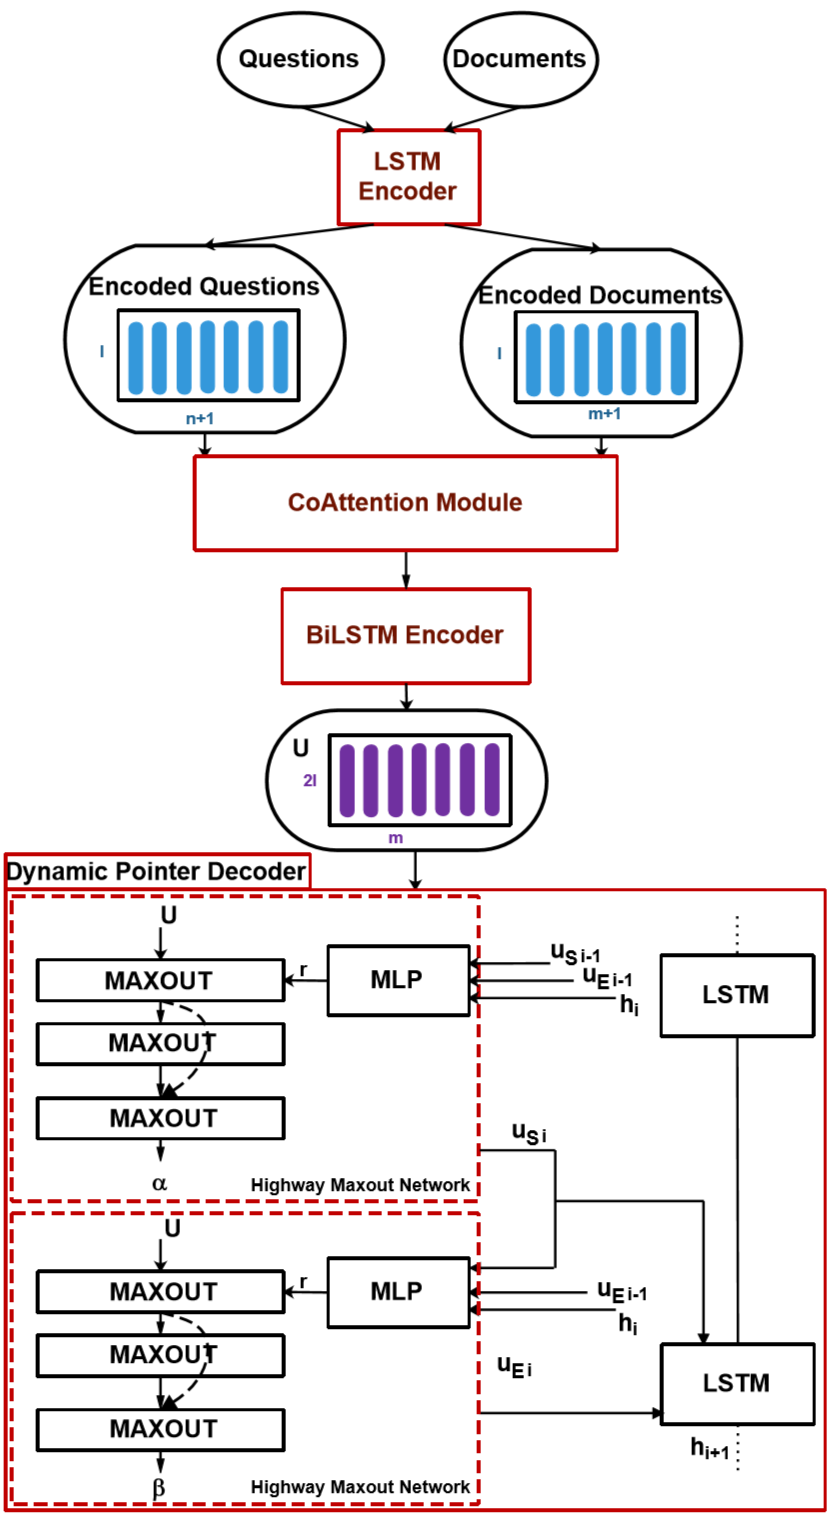
\includegraphics[scale=0.8]{plots/Model_Overview.png}
\caption{Illustration of the network.}
\end{figure}

This section presents the full Dynamic Coattention Network model from \cite{dcn}, that we have reimplemented. The model overview is illustrated in Fig.~\ref{fig:dcn}.

\subsubsection{LSTM Encoder}
This module encodes the documents and questions using the same LSTM. Further, the question encoding is passed through an extra layer (linear transformation followed by $\tanh$) to allow for a difference between document and question encoding spaces.

% I wonder what the point of using the same LSTM is if you later add this extra transformation to Q. Just to have fewer params?

Finally, each of the two encodings is appended a single learned sentinel element at the end, which can be attended to later, which should be interpreted as a `choice to not attend to any particular word'.

\subsubsection{The Coattention Module}

\begin{figure}\label{fig:coattention}
\centering
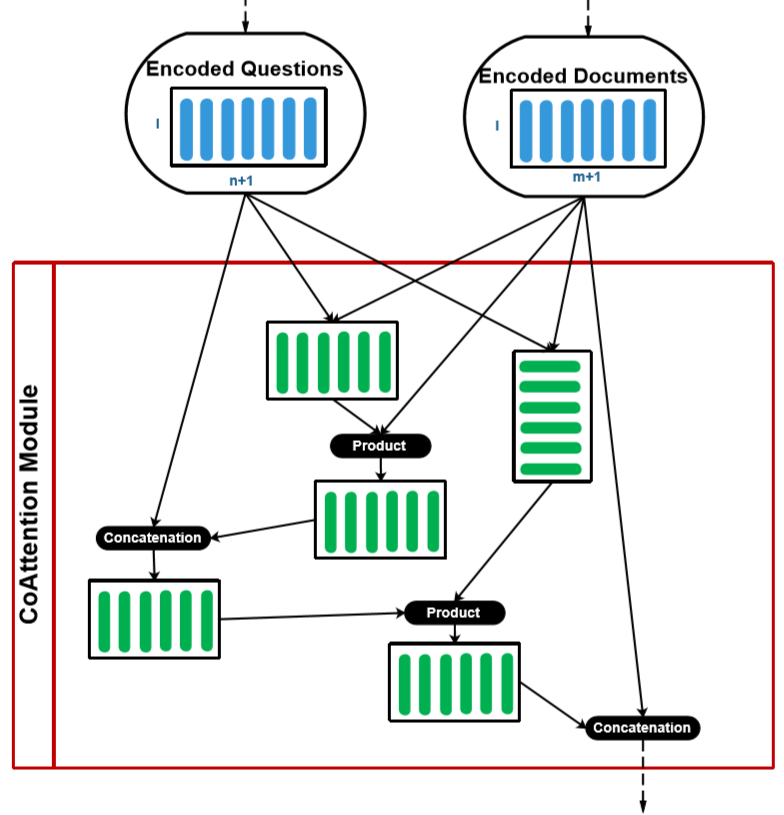
\includegraphics[scale=0.6]{plots/Coattention_Module.png}
\caption{The coattention mechanism.}
\end{figure}

\textit{Coattention}, as used in \cite{dcn} refers to the idea that the question encodings and document encodings each attend to the other, producing two attention-weight matrices (which are, up to a transposition, simply the column-wise and row-wise softmaxes of the product of the two encoding matrices).

In the paper, first the summary of the document $C^Q$ is computed per each word of the question (standard use of attention). Then both that summary and the question encoding itself are multiplied by the other attention matrix, producing a summary of the question (per document word) as well as a summary of $C^Q$.

Both those summaries are concatenated to produce the \textit{coattention context}, of the length equal to document length, which is outputted by the coattention module. The next module also receives the original document encoding. The entire structure of the  is illustrated in Fig.~\ref{fig:coattention}.


\subsubsection{The Bi-LSTM Encoder}

A bidirectional LSTM is used as the final step of the encoder. As the $t^\text{th}$ input it receives the $t^\text{th}$ word of the document, and the $t^\text{th}$ component of the coattention context. The rationale is to combine the temporal information (i.e. word order) with the coattention context.

As a side note, the coattention context itself is already not independent of the word order, because it is built upon the initial (order-sensitive) LSTM encodings of both document and question.


\subsubsection{The Dynamic Pointer Decoder and the loss}

The encoding $U$ produced by the Bi-LSTM encoder is consumed by the Dynamic Pointer Decoder.

The decoder works in an iterative manner, at each iteration outputting a proposed answer span -- i.e. two indices (pointers) indicating a substring of the input document, which is to be interpreted as the predicted answer. The indices are denoted by $E^i$ and $S^i$ in Fig.~\ref{fig:dcn}.

At each iteration, two Highway Maxout Networks (see Section~\ref{sssec:hmn}) take the previous guess\footnote{To be precise, the HMN responsible for predicting the end-pointer gets the old end-prediction but the newest start-prediction available -- in this way the roles of the two HMNs are not symmetric.} (initialised to $(0,0)$), a hidden state and the encoding $U$ into consideration, and produce scores for all start-indices and end-indices. The highest-scoring pair (which could possibly represent an invalid segment by having the start-index be greater than the end-index) is chosen as the next guess. The entire score vectors are used to compute the cross-entropy loss. A new hidden state is then computed by an LSTM, to prepare for the next iteration.

The decoder is described in the original paper to be run until convergence, and the loss is accummulated over all the iterations. 
We note that mathematical convergence is hard to verify, because of the evolving hidden state, and so we interpret that as having a guess $(s,e)$ index-pair repeat twice in a row.


\subsubsection{The Highway Maxout Network}\label{sssec:hmn} \TODOx{Dip, please polish this.}

This module takes the previous encoded start position $u_{s_{i-1}}$ and end position $u_{e_{i-1}}$, the co-attention encoding corresponding to the $t^{th}$ word in the document $u_{t}$, and the current hidden state of the Dynamic Pointer Decoder $h_i$. It returns the start score $\alpha_t$ and end score $\beta_t$ of the $t^{th}$ word in the document.

Most specifically, the module implements the equations (9),(10),(11) and (12) of the paper. \\
We apply nn.CrossEntropy \TODOx{Formatting.} between the predicted spans and the true spans. At first, we did not know that nn.CrossEntropy already performed softmax, and applied softmax twice. 

Furthermore, the predicted spans are found by computing the maximum of the alphas and betas. We first used th.argmax but faced the problem of its non-differentiability. To preserve the integrity of the computation graph we used th.max \TODOx{Formatting.} instead. Hence, all operations are differentiable, and the depth of the graph is determined dynamically.


\section{Our implementation}

\subsection{Model}

We have reimplemented the network from scratch in PyTorch (\cite{pytorch}). We referred to an existing PyTorch implementation\footnote{\url{https://github.com/atulkum/co-attention}} occasionally, due to our prior inexperience with PyTorch, but did not reuse their code (\TODO\ is that accurate -- has anyone copy-pasted code from there? I think a lot of the batching is re-used from the their implementation but i might be wrong \TODOx{ Discuss what to do about this.}).

In some places our implementation differed from the paper's description, or the paper failed to provide details, and we had to make design decisions ourselves. Here are the most notable cases:
\begin{itemize}
\item \TODO\ Dropout
\item \TODO\ Zero padding and interaction with sentinel
\item \TODO\ \ttt{MAX\_ITER=1}
\item \TODO\ Hyperparameters for ADAM
\end{itemize}


\subsection{The training pipeline}

\subsubsection{Word embeddings}
Following the original paper, we use pre-trained word vectors `Glove 840B' from Stanford (\cite{glove}). The set contains $2.2$M word vectors of dimensionality $300$.

\subsubsection{Dataset and preprocessing}
To train our model, we used the SQuAD2.0 dataset (\cite{rajpurkar2018know}). 
Since the dataset represents unanswerable questions as having no ground truth answers, no further work was needed to exclude them during training.
% \TODOx{Dip, how did you achieve that there were no unanswerable questions in the training set?}

To tokenise the data, we used Stanford CoreNLP (\cite{coreNLP}). We convert the character-indexed answer spans from SQuAD2.0 to token indexing.

The conversion was simplified by disabling Penn Treebank token transformations\footnote{See \url{https://nlp.stanford.edu/software/tokenizer.shtml}.} to prevent having some tokens replaced by longer placeholders. Despite this, there were still special cases in which the conversion could not be completed, which we excluded from training and evaluation. \TODOx{Example where character-to-token index conversion failed}

We group the data into batches of size $64$ for efficient training.

\subsubsection{Training}
We use the ADAM optimiser (\cite{adam}), following the original paper. An implementation of ADAM is provided by PyTorch and we set the learning rate to \ttt{lr = 0.001}.

Custom infrastructure code we have written automates periodic saving of the trained model to a session directory and allows for easily resuming any training session later on. We also keep track of how the loss evolves, in an append-only log file.

We run the training on a single \TODO\ GPU for \TODO\ steps, which constitutes \TODO\ epochs (the dataset size is \TODO).

\TODO\ Insert some loss (or loss+score) plots.

\section{Experimental results}

\TODO\ Insert tables and plots of our model's performance, compared with the values reported in the original paper.

% What did we evaluate

We trained an implementation of the DCN with the decoder performing only one iteration, and no dropout. 

% Hyperparameters and training time
We trained it using Adam with a learning rate of $0.001$ for 23 epochs (corresponding to 23 passes over the entire training set).
We stopped training as soon as we observed that model's F1 score on the dev set no longer increased, despite the training loss continuing to decrease (Figure~\TODO\textbf{})

\begin{table}[h]
\begin{center}
\begin{tabular}{l c c c c}
\toprule
Model                                           & Dev EM        & Dev F1 \\
\midrule
DCN with single iteration decoder (Ours)        &               &     \\
DCN with single iteration decoder (\cite{dcn})  & 63.7          & 74.0\\
\bottomrule
\end{tabular}
\end{center}
\caption{Performance of our main model on the SQuAD dataset (i.e.\ performance on the answerable questions in the SQuAD 2.0 dataset).}
\label{table:main-results}
\end{table}

Table~\ref{table:main-results} summarises the performance of this model, compared to the closest comparable model studied by~\cite{dcn} (the DCN with single iteration).

\textbf{Performance across length}

\textbf{Breakdown of F1 distribution}

\subsection{Conclusions}

\TODO\ State we have failed to reproduce the performance stated in the paper. Present some hypotheses why.

\section{Findings}

\TODO\ Interesting findings/experiments made throughout implementation/training that do not fit into the previous Section.


\section{Cost of reproducing the paper}

% find . -name '*.py' | xargs wc -l | sort -nr
A total of 3375 lines of Python code were written for this project and over 350 git commits were submitted into our development repository. Initial implementation of the model and training pipeline took about two weeks. Further, debugging until we managed to get significant learning done took more than an extra week of intense work.

We would loosely estimate the total number of work-hours spent on the project (excluding the report and poster) by the 5 team members to be about \TODOx{200?}.

We have not had to contact the paper's authors.
We have used a single privately-owned RTX 2060 SUPER GPU with 8GB of RAM for training and evaluation. We have found that we could have two training sessions running simultaneously if the multiple iterations option was disabled in the network.

\TODOx{Mention how much memory was taken up by the loaded embeddings. Theoretically the multiple models being trained in parallel could only use a single shared embeddings set.}

\subsection{Failures to reproduce the paper exactly}
\TODO\ Describe any parts of the paper that we didn't reproduce, and estimate whether that would have been difficult/time-consuming.

\TODO\ \textit{Optional. State largest roadblocks we've faced and how we've overcome them in the end.}

\bibliography{refs}

\end{document}